%!TeX root=../pridetop.tex
\chapter[Chapter \thechapter]{}
	
	
\begin{figure}[t!]
\centering
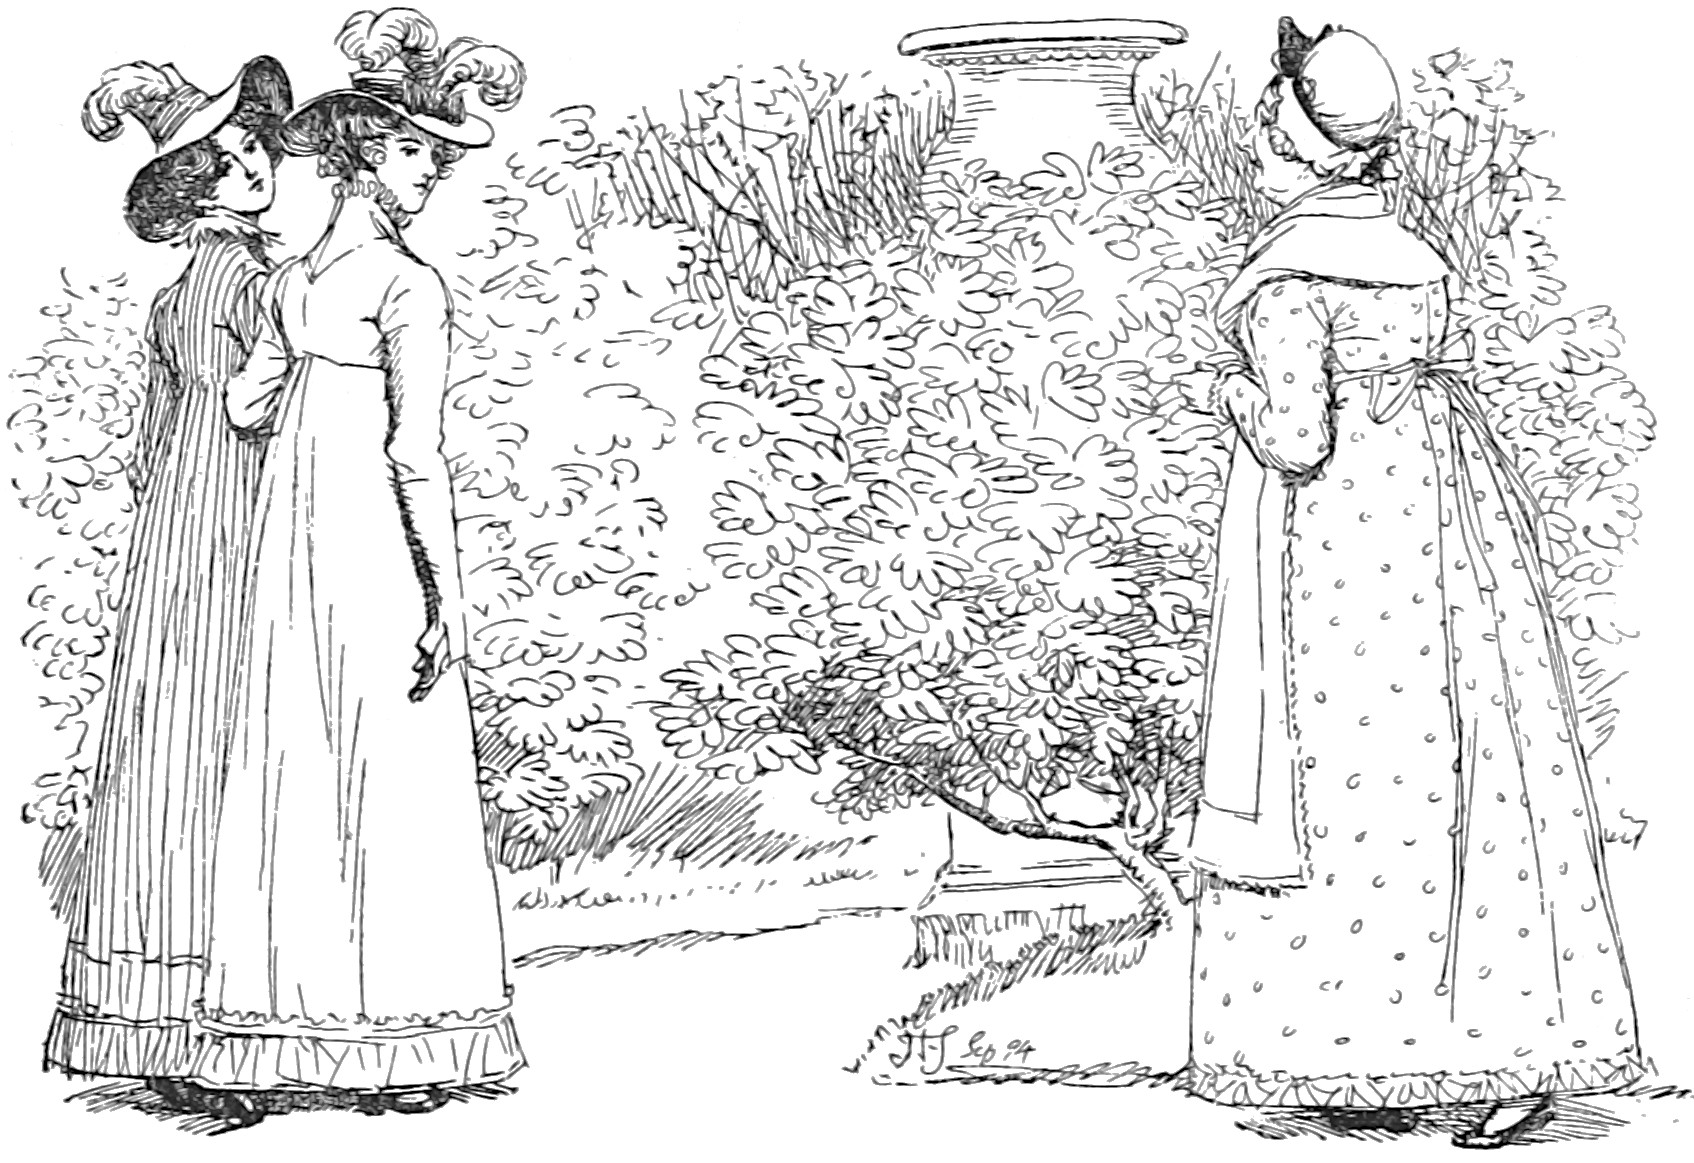
\includegraphics[width=.8\linewidth]{49top}
\captionlistentry{Headpiece to Chapter \thechapter}
\end{figure}


\lettrine[lines=6,image=true]{initials/chap49t}{wo}  days after Mr Bennet's return, as Jane and Elizabeth were walking together in the shrubbery behind the house, they saw the housekeeper coming towards them, and concluding that she came to call them to their mother, went forward to meet her; but instead of the expected summons, when they approached her, she said to Miss Bennet, »I beg your pardon, madam, for interrupting you, but I was in hopes you might have got some good news from town, so I took the liberty of coming to ask.«

»What do you mean, Hill? We have heard nothing from town.«

»Dear madam,« cried Mrs Hill, in great astonishment, »don't you know there is an express come for master from Mr Gardiner? He has been here this half hour, and master has had a letter.«

Away ran the girls, too eager to get in to have time for speech. They ran through the vestibule into the breakfast-room; from thence to the library;—their father was in neither; and they were on the point of seeking him upstairs with their mother, when they were met by the butler, who said,—

»If you are looking for my master, ma'am, he is walking towards the little copse.«

Upon this information, they instantly passed through the hall once more, and ran across the lawn after their father, who was deliberately pursuing his way towards a small wood on one side of the paddock.

Jane, who was not so light, nor so much in the habit of running as Elizabeth, soon lagged behind, while her sister, panting for breath, came up with him, and eagerly cried out,—

»Oh, papa, what news? what news? have you heard from my uncle?«

»Yes, I have had a letter from him by express.«

»Well, and what news does it bring—good or bad?«

\begin{figure}[tbh]
\centering

\includegraphics[width=.8\linewidth]{49readit}
\captionlistentry{»Perhaps you would like to read it«}
\end{figure}

»What is there of good to be expected?« said he, taking the letter from his pocket; »but perhaps you would like to read it.«

Elizabeth impatiently caught it from his hand. Jane now came up.

»Read it aloud,« said their father, »for I hardly know myself what it is about.«

\begin{quotation}
	
\begin{flushright}
Gracechurch Street\\ Monday, August 2.
\end{flushright}

\noindent My dear Brother,

At last I am able to send you some tidings of my niece, and such as, upon the whole, I hope will give you satisfaction. Soon after you left me on Saturday, I was fortunate enough to find out in what part of London they were. The particulars I reserve till we meet. It is enough to know they are discovered: I have seen them both—
\end{quotation}

»Then it is as I always hoped,« cried Jane: »they are married!«

Elizabeth read on: 

\begin{quotation}

I have seen them both. They are not married, nor can I find there was any intention of being so; but if you are willing to perform the engagements which I have ventured to make on your side, I hope it will not be long before they are. All that is required of you is, to assure to your daughter, by settlement, her equal share of the five thousand pounds, secured among your children after the decease of yourself and my sister; and, moreover, to enter into an engagement of allowing her, during your life, one hundred pounds per annum. These are conditions which, considering everything, I had no hesitation in complying with, as far as I thought myself privileged, for you. I shall send this by express, that no time may be lost in bringing me your answer. You will easily comprehend, from these particulars, that Mr Wickham's circumstances are not so hopeless as they are generally believed to be. The world has been deceived in that respect; and I am happy to say, there will be some little money, even when all his debts are discharged, to settle on my niece, in addition to her own fortune. If, as I conclude will be the case, you send me full powers to act in your name throughout the whole of this business, I will immediately give directions to Haggerston for preparing a proper settlement. There will not be the smallest occasion for your coming to town again; therefore stay quietly at Longbourn, and depend on my diligence and care. Send back your answer as soon as you can, and be careful to write explicitly. We have judged it best that my niece should be married from this house, of which I hope you will approve. She comes to us to-day. I shall write again as soon as anything more is determined on. Yours, etc.

\begin{flushright}\scshape
Edw. Gardiner.
\end{flushright}

\end{quotation}

»Is it possible?« cried Elizabeth, when she had finished. »Can it be possible that he will marry her?«

»Wickham is not so undeserving, then, as we have thought him,« said her sister. »My dear father, I congratulate you.«

»And have you answered the letter?« said Elizabeth.

»No; but it must be done soon.«

Most earnestly did she then entreat him to lose no more time before he wrote.

»Oh! my dear father,« she cried, »come back and write immediately. Consider how important every moment is in such a case.«

»Let me write for you,« said Jane, »if you dislike the trouble yourself.«

»I dislike it very much,« he replied; »but it must be done.«

And so saying, he turned back with them, and walked towards the house.

»And—may I ask?« said Elizabeth; »but the terms, I suppose, must be complied with.«

»Complied with! I am only ashamed of his asking so little.«

»And they \textit{must} marry! Yet he is \textit{such} a man.«

»Yes, yes, they must marry. There is nothing else to be done. But there are two things that I want very much to know:—one is, how much money your uncle has laid down to bring it about; and the other, how I am ever to pay him.«

»Money! my uncle!« cried Jane, »what do you mean, sir?«

»I mean that no man in his proper senses would marry Lydia on so slight a temptation as one hundred a year during my life, and fifty after I am gone.«

»That is very true,« said Elizabeth; »though it had not occurred to me before. His debts to be discharged, and something still to remain! Oh, it must be my uncle's doings! Generous, good man, I am afraid he has distressed himself. A small sum could not do all this.«

»No,« said her father. »Wickham's a fool if he takes her with a farthing less than ten thousand pounds: I should be sorry to think so ill of him, in the very beginning of our relationship.«

»Ten thousand pounds! Heaven forbid! How is half such a sum to be repaid?«

Mr Bennet made no answer; and each of them, deep in thought, continued silent till they reached the house. Their father then went to the library to write, and the girls walked into the breakfast-room.

»And they are really to be married!« cried Elizabeth, as soon as they were by themselves. »How strange this is! and for \textit{this} we are to be thankful. That they should marry, small as is their chance of happiness, and wretched as is his character, we are forced to rejoice! Oh, Lydia!«

»I comfort myself with thinking,« replied Jane, »that he certainly would not marry Lydia, if he had not a real regard for her. Though our kind uncle has done something towards clearing him, I cannot believe that ten thousand pounds, or anything like it, has been advanced. He has children of his own, and may have more. How could he spare half ten thousand pounds?«

»If we are ever able to learn what Wickham's debts have been,« said Elizabeth, »and how much is settled on his side on our sister, we shall exactly know what Mr Gardiner has done for them, because Wickham has not sixpence of his own. The kindness of my uncle and aunt can never be requited. Their taking her home, and affording her their personal protection and countenance, is such a sacrifice to her advantage as years of gratitude cannot enough acknowledge. By this time she is actually with them! If such goodness does not make her miserable now, she will never deserve to be happy! What a meeting for her, when she first sees my aunt!«

»We must endeavour to forget all that has passed on either side,« said Jane: »I hope and trust they will yet be happy. His consenting to marry her is a proof, I will believe, that he is come to a right way of thinking. Their mutual affection will steady them; and I flatter myself they will settle so quietly, and live in so rational a manner, as may in time make their past imprudence forgotten.«

»Their conduct has been such,« replied Elizabeth, »as neither you, nor I, nor anybody, can ever forget. It is useless to talk of it.«

It now occurred to the girls that their mother was in all likelihood perfectly ignorant of what had happened. They went to the library, therefore, and asked their father whether he would not wish them to make it known to her. He was writing, and, without raising his head, coolly replied,—

»Just as you please.«

»May we take my uncle's letter to read to her?«

»Take whatever you like, and get away.«

Elizabeth took the letter from his writing-table, and they went upstairs together. Mary and Kitty were both with Mrs Bennet: one communication would, therefore, do for all. After a slight preparation for good news, the letter was read aloud. Mrs Bennet could hardly contain herself. As soon as Jane had read Mr Gardiner's hope of Lydia's being soon married, her joy burst forth, and every following sentence added to its exuberance. She was now in an irritation as violent from delight as she had ever been fidgety from alarm and vexation. To know that her daughter would be married was enough. She was disturbed by no fear for her felicity, nor humbled by any remembrance of her misconduct.

»My dear, dear Lydia!« she cried: »this is delightful indeed! She will be married! I shall see her again! She will be married at sixteen! My good, kind brother! I knew how it would be—I knew he would manage everything. How I long to see her! and to see dear Wickham too! But the clothes, the wedding clothes! I will write to my sister Gardiner about them directly. Lizzy, my dear, run down to your father, and ask him how much he will give her. Stay, stay, I will go myself. Ring the bell, Kitty, for Hill. I will put on my things in a moment. My dear, dear Lydia! How merry we shall be together when we meet!«

Her eldest daughter endeavoured to give some relief to the violence of these transports, by leading her thoughts to the obligations which Mr Gardiner's behaviour laid them all under.

»For we must attribute this happy conclusion,« she added, »in a great measure to his kindness. We are persuaded that he has pledged himself to assist Mr Wickham with money.«

»Well,« cried her mother, »it is all very right; who should do it but her own uncle? If he had not had a family of his own, I and my children must have had all his money, you know; and it is the first time we have ever had anything from him except a few presents. Well! I am so happy. In a short time, I shall have a daughter married. Mrs Wickham! How well it sounds! And she was only sixteen last June. My dear Jane, I am in such a flutter, that I am sure I can't write; so I will dictate, and you write for me. We will settle with your father about the money afterwards; but the things should be ordered immediately.«

She was then proceeding to all the particulars of calico, muslin, and cambric, and would shortly have dictated some very plentiful orders, had not Jane, though with some difficulty, persuaded her to wait till her father was at leisure to be consulted. One day's delay, she observed, would be of small importance; and her mother was too happy to be quite so obstinate as usual. Other schemes, too, came into her head.

»I will go to Meryton,« said she, »as soon as I am dressed, and tell the good, good news to my sister Philips. And as I come back, I can call on Lady Lucas and Mrs Long. Kitty, run down and order the carriage. An airing would do me a great deal of good, I am sure. Girls, can I do anything for you in Meryton? Oh! here comes Hill. My dear Hill, have you heard the good news? Miss Lydia is going to be married; and you shall all have a bowl of punch to make merry at her wedding.«

Mrs Hill began instantly to express her joy. Elizabeth received her congratulations amongst the rest, and then, sick of this folly, took refuge in her own room, that she might think with freedom. Poor Lydia's situation must, at best, be bad enough; but that it was no worse, she had need to be thankful. She felt it so; and though, in looking forward, neither rational happiness, nor worldly prosperity could be justly expected for her sister, in looking back to what they had feared, only two hours ago, she felt all the advantages of what they had gained.